%File: anonymous-submission-latex-2026.tex
\documentclass[letterpaper]{article} % DO NOT CHANGE THIS
\usepackage[submission]{aaai2026}  % DO NOT CHANGE THIS
\usepackage{times}  % DO NOT CHANGE THIS
\usepackage{helvet}  % DO NOT CHANGE THIS
\usepackage{courier}  % DO NOT CHANGE THIS
\usepackage[hyphens]{url}  % DO NOT CHANGE THIS
\usepackage{graphicx} % DO NOT CHANGE THIS
\urlstyle{rm} % DO NOT CHANGE THIS
\def\UrlFont{\rm}  % DO NOT CHANGE THIS
\usepackage{natbib}  % DO NOT CHANGE THIS AND DO NOT ADD ANY OPTIONS TO IT
\usepackage{caption} % DO NOT CHANGE THIS AND DO NOT ADD ANY OPTIONS TO IT
\frenchspacing  % DO NOT CHANGE THIS
\setlength{\pdfpagewidth}{8.5in} % DO NOT CHANGE THIS
\setlength{\pdfpageheight}{11in} % DO NOT CHANGE THIS
%
% These are recommended to typeset algorithms but not required. See the subsubsection on algorithms. Remove them if you don't have algorithms in your paper.
\usepackage{algorithm}
\usepackage{algorithmic}

%
% These are are recommended to typeset listings but not required. See the subsubsection on listing. Remove this block if you don't have listings in your paper.
\usepackage{newfloat}
\usepackage{listings}
\DeclareCaptionStyle{ruled}{labelfont=normalfont,labelsep=colon,strut=off} % DO NOT CHANGE THIS
\lstset{%
	basicstyle={\footnotesize\ttfamily},% footnotesize acceptable for monospace
	numbers=left,numberstyle=\footnotesize,xleftmargin=2em,% show line numbers, remove this entire line if you don't want the numbers.
	aboveskip=0pt,belowskip=0pt,%
	showstringspaces=false,tabsize=2,breaklines=true}
\floatstyle{ruled}
\newfloat{listing}{tb}{lst}{}
\floatname{listing}{Listing}
%
% Keep the \pdfinfo as shown here. There's no need
% for you to add the /Title and /Author tags.
\pdfinfo{
/TemplateVersion (2026.1)
}

% DISALLOWED PACKAGES
% \usepackage{authblk} -- This package is specifically forbidden
% \usepackage{balance} -- This package is specifically forbidden
% \usepackage{color (if used in text)
% \usepackage{CJK} -- This package is specifically forbidden
% \usepackage{float} -- This package is specifically forbidden
% \usepackage{flushend} -- This package is specifically forbidden
% \usepackage{fontenc} -- This package is specifically forbidden
% \usepackage{fullpage} -- This package is specifically forbidden
% \usepackage{geometry} -- This package is specifically forbidden
% \usepackage{grffile} -- This package is specifically forbidden
% \usepackage{hyperref} -- This package is specifically forbidden
% \usepackage{navigator} -- This package is specifically forbidden
% (or any other package that embeds links such as navigator or hyperref)
% \indentfirst} -- This package is specifically forbidden
% \layout} -- This package is specifically forbidden
% \multicol} -- This package is specifically forbidden
% \nameref} -- This package is specifically forbidden
% \usepackage{savetrees} -- This package is specifically forbidden
% \usepackage{setspace} -- This package is specifically forbidden
% \usepackage{stfloats} -- This package is specifically forbidden
% \usepackage{tabu} -- This package is specifically forbidden
% \usepackage{titlesec} -- This package is specifically forbidden
% \usepackage{tocbibind} -- This package is specifically forbidden
% \usepackage{ulem} -- This package is specifically forbidden
% \usepackage{wrapfig} -- This package is specifically forbidden
% DISALLOWED COMMANDS
% \nocopyright -- Your paper will not be published if you use this command
% \addtolength -- This command may not be used
% \balance -- This command may not be used
% \baselinestretch -- Your paper will not be published if you use this command
% \clearpage -- No page breaks of any kind may be used for the final version of your paper
% \columnsep -- This command may not be used
% \newpage -- No page breaks of any kind may be used for the final version of your paper
% \pagebreak -- No page breaks of any kind may be used for the final version of your paperr
% \pagestyle -- This command may not be used
% \tiny -- This is not an acceptable font size.
% \vspace{- -- No negative value may be used in proximity of a caption, figure, table, section, subsection, subsubsection, or reference
% \vskip{- -- No negative value may be used to alter spacing above or below a caption, figure, table, section, subsection, subsubsection, or reference
\usepackage{amsmath}
\usepackage{amsfonts}
\usepackage{amssymb}
\usepackage{amsthm}

\setcounter{secnumdepth}{1} %May be changed to 1 or 2 if section numbers are desired.

% The file aaai2026.sty is the style file for AAAI Press
% proceedings, working notes, and technical reports.
%

% Title

% Your title must be in mixed case, not sentence case.
% That means all verbs (including short verbs like be, is, using,and go),
% nouns, adverbs, adjectives should be capitalized, including both words in hyphenated terms, while
% articles, conjunctions, and prepositions are lower case unless they
% directly follow a colon or long dash
\title{Learning Mission-Time Linear Temporal Logic from Positive and Negative Data}
% \author{
%     %Authors
%     % All authors must be in the same font size and format.
%     Written by AAAI Press Staff\textsuperscript{\rm 1}\thanks{With help from the AAAI Publications Committee.}\\
%     AAAI Style Contributions by Pater Patel Schneider,
%     Sunil Issar,\\
%     J. Scott Penberthy,
%     George Ferguson,
%     Hans Guesgen,
%     Francisco Cruz\equalcontrib,
%     Marc Pujol-Gonzalez\equalcontrib
% }
% \affiliations{
%     %Afiliations
%     \textsuperscript{\rm 1}Association for the Advancement of Artificial Intelligence\\
%     % If you have multiple authors and multiple affiliations
%     % use superscripts in text and roman font to identify them.
%     % For example,

%     % Sunil Issar\textsuperscript{\rm 2},
%     % J. Scott Penberthy\textsuperscript{\rm 3},
%     % George Ferguson\textsuperscript{\rm 4},
%     % Hans Guesgen\textsuperscript{\rm 5}
%     % Note that the comma should be placed after the superscript

%     1101 Pennsylvania Ave, NW Suite 300\\
%     Washington, DC 20004 USA\\
%     % email address must be in roman text type, not monospace or sans serif
%     proceedings-questions@aaai.org
% %
% % See more examples next
% }

%Example, Single Author, ->> remove \iffalse,\fi and place them surrounding AAAI title to use it
\iffalse
\title{My Publication Title --- Single Author}
\author {
    Author Name
}
\affiliations{
    Affiliation\\
    Affiliation Line 2\\
    name@example.com
}
\fi

\iffalse
%Example, Multiple Authors, ->> remove \iffalse,\fi and place them surrounding AAAI title to use it
\title{My Publication Title --- Multiple Authors}
\author {
    % Authors
    First Author Name\textsuperscript{\rm 1},
    Second Author Name\textsuperscript{\rm 2},
    Third Author Name\textsuperscript{\rm 1}
}
\affiliations {
    % Affiliations
    \textsuperscript{\rm 1}Affiliation 1\\
    \textsuperscript{\rm 2}Affiliation 2\\
    firstAuthor@affiliation1.com, secondAuthor@affilation2.com, thirdAuthor@affiliation1.com
}
\fi


\begin{document}
% PAGE LIMIT: 7 PAGES PLUS ADDITIONAL PAGES FOR REFERENCES

\maketitle

\begin{abstract}
AAAI creates proceedings, working notes, and technical reports directly from electronic source furnished by the authors. To ensure that all papers in the publication have a uniform appearance, authors must adhere to the following instructions.
\end{abstract}

% Uncomment the following to link to your code, datasets, an extended version or similar.
% You must keep this block between (not within) the abstract and the main body of the paper.
% \begin{links}
%     \link{Code}{https://aaai.org/example/code}
%     \link{Datasets}{https://aaai.org/example/datasets}
%     \link{Extended version}{https://aaai.org/example/extended-version}
% \end{links}

\section{Introduction}
\label{sec:intro}

The task of learning temporal logic specifications from data has wide applications in a variety of domains, such as specification mining, model checking, runtime verification, and inferring reinforcement learning objectives. 
Given a collection of desirable and undesirable behaviors of a system, i.e., positive and negative examples, we study the problem of learning a temporal logic formula that succinctly captures the system behavior.

In this technical report, we focus on learning Mission-time Linear Temporal Logic (MLTL) formulas from positive and negative examples.
MLTL is a discrete time, finite interval bounded variant of the popular Linear Temporal Logic (LTL) \cite{Pnueli77}, and we provide a brief overview of MLTL in Section \ref{sec:mltl}.
We describe five differing approaches to MLTL inference: grammar evolution, informed beam search, deep learning via transformers, template-driven search, and Bayesian network structure learning.
We also evaluate the performance of these approaches on a set of synthetic datasets of varying complexity.
Grammar evolution and informed beam search yielded promising results across all datasets, while template-driven search was only able to learn simple formulas.
Deep learning via transformers encountered significant challenges in training, and Bayesian network structure learning led to theoretical results that does not yet yield a practical algorithm for MLTL inference, but has use in other applications.

Work in learning temporal logic formulas have also recently been explored, with approaches ranging from symbolic learning algorithms \cite{roy_ltlf_learning} \cite{camacho_ltlf_learning} to deep learning algorithms \cite{stl_learning},\cite{Luo_Liang_Du_Wan_Peng_Zhang_2022}.
There is no published work on learning MLTL formulas, and the goal of this project is to explore various approaches to this problem, and to compare and contrast their performance.


\section{Mission-time Linear Temporal Logic}
\label{sec:mltl}

MLTL is a discrete time, finite interval bounded temporal logic that has found numerous recent applications. 
For example, MLTL was the specification logic for NASA's Robonaut2 verification project \cite{KZJZR20}, as well as for the design-time and runtime verification of the NASA Lunar Gateway Vehicle System Manager \cite{DBR21}.
Other applications of MLTL include autonomous satellite \cite{JAXA}, UAV Traffic Management \cite{HCHJR21}, and more \cite{HLR21}, \cite{LLR21}, \cite{LJBHCLR22}, \cite{AJR22}. 

\subsection{Syntax and Semantics}
The syntax of MLTL for a finite set of atomic propositions $\mathcal{AP}$ is defined as: 
$$ 
\xi := 
true \ | 
\ false \ | 
\ p \ | 
\ \neg \phi \ | 
\ \phi \land \psi \ | 
\ \phi \lor \psi \ | 
\ \mathcal{F}_{[a,b]} \phi \ | 
\ \mathcal{G}_{[a,b]} \phi \ | 
\ \phi \mathcal{U}_{[a,b]} \psi \ | 
\ \phi \mathcal{R}_{[a,b]} \psi, 
$$
where $p \in \mathcal{AP}$, $a, b \in \mathbb{Z}$ such that $0 \leq a \leq b$, and $\phi$, $\psi$, $\xi$ are MLTL formulas. 
The symbols $\mathcal{F},\mathcal{G},\mathcal{U},\mathcal{R}$ denote the temporal operators Future, Globally, Until, and Release, respectively.

\textbf{Definition}
    A \textbf{trace} over a finite set of atomic propositions $\mathcal{AP}$ is a finite sequence $\pi = \pi[0], \pi[1], ..., \pi[k-1]$, where each $\pi[i] \subseteq \mathcal{AP}$. 

A trace represents an assignment to the truth values of each atomic proposition over time, where $p \in \mathcal{AP}$ holds at time $i$ if and only if $p \in \pi[i]$. 
We denote the length of a trace $\pi$ as $|\pi|$, and denote the suffix of a trace $\pi$ starting at, and including, $i$ as $\pi_i$.
Thus note that $\pi_0 = \pi$. 

\begin{figure}[h]
\centering
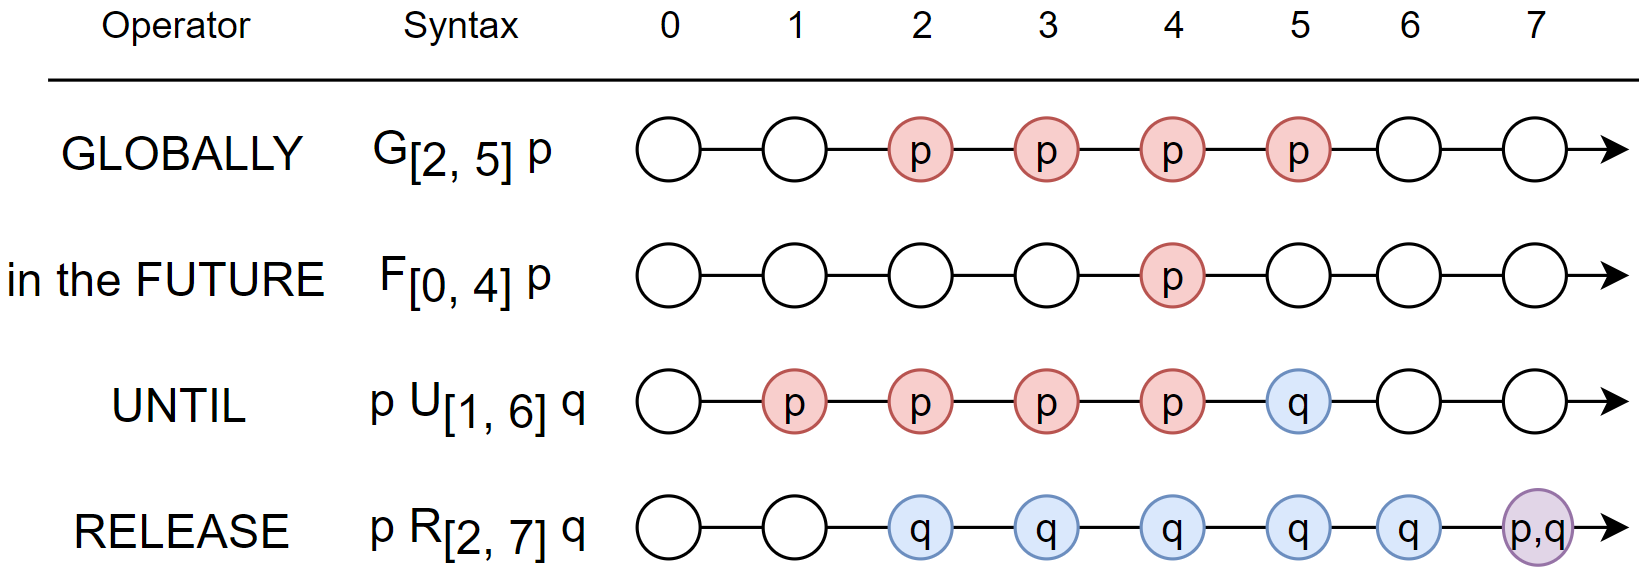
\includegraphics[width=\linewidth]{figs/temporal_operators.png}
\caption{``Intuitive'' semantics of the temporal operators. The presence of a variable indicates that it is true at that time step, and the absence indicates that it is false.}
\label{fig:temporal_operators}
\end{figure}


A trace $\pi$ \textbf{satisfies} MLTL formula $\phi$, denoted $\pi \vDash \phi$, is defined as follows:
\begin{minipage}{0.5\textwidth}
\begin{flalign*}
    &\pi \vDash p \text{ iff } p \in \pi[0]&\\
    &\pi \vDash \alpha \land \beta \text{ iff } \pi \vDash \alpha \text{ and } \pi \vDash \beta&
\end{flalign*}
\end{minipage}
\begin{minipage}{0.5\textwidth}
\begin{flalign*}
    &\pi \vDash \neg \alpha \text{ iff } \pi \nvDash \alpha&\\
    &\pi \vDash \alpha \lor \beta \text{ iff } \pi \vDash \alpha \text{ or } \pi \vDash \beta&
\end{flalign*}
\end{minipage}
{\setlength{\abovedisplayskip}{0pt}
\begin{flalign*}
    &\pi \vDash \mathcal{F}_{[a,b]}\alpha \text{ iff } |\pi| > a \text{ and } \exists i \in [a,b] \text{ such that } \pi_i \vDash \alpha&\\
    &\pi \vDash \mathcal{G}_{[a,b]}\alpha \text{ iff } |\pi| \leq a \text{ or } \forall i \in [a,b] \ \pi_i \vDash \alpha&\\
    &\pi \vDash \alpha \ \mathcal{U}_{[a,b]} \beta \text{ iff } |\pi| > a \text{ and } \exists i \in [a,b] \text{ such that } \pi_i \vDash \beta \text{ and }\forall j \in [a, i-1]\ \pi_j \vDash \alpha &\\
    &\pi \vDash \alpha \ \mathcal{R}_{[a,b]} \beta \text{ iff } |\pi| \leq a \text{ or } (\forall i \in [a,b] \ \pi_i \vDash \beta) \text{ or }(\exists j \in [a,b-1] \text{ such that } \pi_j \vDash \alpha &\\
    &\indent \text{ and } \forall a \leq k \leq j \ \pi_k \vDash \beta)&
\end{flalign*}}

Illustrations of the intuitive meanings of the temporal operators appear in Figure \ref{fig:temporal_operators}.
Two MLTL formulas $\phi$ and $\psi$ are semantically equivalent if for any trace $\pi$, $\pi \vDash \phi \iff \pi \vDash \psi$.
As in LTL, the usual dual equivalence relationships hold between the Finally and Globally operators, and the Until and Release operators.
That is, $\mathcal{F}_{[a,b]}\alpha \equiv \neg \mathcal{G}_{[a,b]}\neg \alpha$ and $\alpha \ \mathcal{U}_{[a,b]} \beta \equiv \neg (\neg \alpha \ \mathcal{R}_{[a,b]} \neg \beta)$.

MLTL reasons over a finite set of atomic propositions, and thus we may assume without loss of generality that $\mathcal{AP} = \{p_0, p_1, \ldots, p_{n-1}\}$.
This imposes a natural ordering on the atomic propositions, which we use to define the string encoding of a trace.

    The \textbf{string encoding}, as defined in \cite{WEST_tool}, of a finite trace $\pi$ of length $m = |\pi|$ over $n = |\mathcal{AP}|$ atomic propositions is the string $w_{\pi} \in \{\textbf{0}, \textbf{1}\}^{mn}$, i.e., a binary string of length $mn$, such that $p_k \in \pi[i]$ if and only if 
    the $(i*n + k)$-th character (indexing from 0) % \footnote{As is standard convention, we use $0$ indexing for the characters of the string.} 
    of $w_{\pi}$ is \textbf{1}.

As an example, for $\mathcal{AP} = {p0, p1}$, the string encoding of the trace $\pi = {p0}, {p0, p1}, {}$ is the binary string $w_\pi = \textbf{10}, \textbf{11}, \textbf{00}$.
The string encoding of traces gives a convenient way to represent traces as binary strings, and also lends MLTL to analysis using formal language theory. 

    The \textbf{future reach} of an MLTL formula $\xi$, denoted $FR(\xi)$, is recursively defined as:
    $$
    FR(\xi) = 
    \begin{cases}
        1 & \text{if } \xi \text{ is an atomic proposition } p \in \mathcal{AP}\\
        FR(\phi) + FR(\psi) & \text{if } \xi = \phi \land \psi \text{ or } \xi = \phi \lor \psi\\
        b + FR(\phi) & \text{if } \xi = \mathcal{F}_{[a,b]}\phi \text{ or } \xi = \mathcal{G}_{[a,b]}\phi\\
        \xi = \max(FR(\phi), FR(\psi)) & \text{if } \xi = \phi \mathcal{U}_{[a,b]} \psi \text{ or } \xi = \phi \mathcal{R}_{[a,b]} \psi
    \end{cases}
    $$

Note that the future reach of an MLTL formula follows the same definition as the worst propagation delay (wpd) of an LTL formula \cite{KZJZR20}. 
Intuitively, the future reach of an MLTL formula is the maximum number of time steps that the formula can specify behavior over.


\section{Learning MLTL from Positive and Negative Data}


\section{Experimental Results}


\section{Discussion and Conclusion}


\appendix
\section{Reference Examples}
\label{sec:reference_examples}

\section{Acknowledgments}


\bibliography{aaai2026}

\end{document}
